\subsection{User Trust} \label{sec:trust}
    In designing assurances that affect trust-based user behaviors, it is critical to know what drives those behaviors. Therefore, some time must be spent on understanding trust. Trust is critical in interpersonal relationships, and it affects the dynamics of intelligent multi-agent systems as simple as one-on-one personal interactions  \cite{Lewicki2006-hj}, to more complicated ones such as financial markets and governments \cite{Fukuyama1995-un}. Consequently, researchers in psychology, sociology, and economics have historically sought to understand the fundamental principles of trust~\cite{Gambetta1988-pi}. Moral philosophers have also thought intently about the topic \cite{Baier1986-im}. Because of interest spanning many disciplines, it is difficult (if not impossible) to write a succinct definition of trust that would completely satisfy all interested parties. Besides that, trust is actually a very broad concept that evades concise definitions at a high level. However, the following adapted definition is broad enough to avoid too much contention \cite{McKnight2004-vv}:

    \begin{description}
        \item [Trust:] a psychological state in which an agent willingly and securely becomes vulnerable, or depends on, a trustee (e.g., another person, institution, or an AIA), having taken into consideration the characteristics (e.g., benevolence, integrity, competence) of the trustee.
    \end{description}

    \subsubsection{Trust between AIAs and humans?}
        Trust is generally understood to exist between people. Is it possible for a human to enter into a trusting relationship with an AIA? That humans actually do feel trust towards machines has been %%% -- surveys not the same as `experimentally' determined...
confirmed several times in research using common subjective psychological questionnaires. Some examples include: \citet{Muir1996-gt,Reeves1997-ad,Groom2007-bz,Mcknight2011-gv,Riley1996-qm,Bainbridge2011-pl,Kaniarasu2012-mo,Salem2015-md,Desai2012-rc, Freedy2007-sg, Inagaki1998-cl, Kaniarasu2013-ho}, and \citet{Wang2016-id}. Several academic experiments have also investigated the possibility of trust existing between humans and (according to the terminology of this survey) AIAs.  All found that some level of trust can be formed in such relationships. For instance, \citet{Lacher2014-yc} points out that people trust an AIA at different levels. As an example, an operator would have different perspectives on trust based on their level of interaction with the AIA. The designer of an AIA would also trust the AIA differently than an end user, due to the differing nature of the trust relationship from one to the other. 

\citet{Tripp2011-rx} investigate the variation of trust between humans and different levels of technology. They experimented with three different levels of technology: Microsoft Access, a recommender system, and Facebook. They found that `human-like' trust applied more to Facebook, while `system-like' trust applied more to MS Access. They conclude that if the system is `human enough', then a human trust model is appropriate. While there is technically a difference between their definitions of `human' and `system' trust we argue that, for practitioners, the differences are negligible. As an example, Tripp, et al suggest replacing the `competence' dimension of the human trust model described below with one called `functionality' that has the same essential definition as competence, except that it accounts for reduced system complexity.

Therefore, in the interest of simplicity we will use a human trust model as a basis for human-AIA trust -- with the understanding that the definitions of the model must correspondingly vary with the complexity of the AIA.

\subsubsection{A Model of Human-AIA Trust}
        We now present a model of human trust, which will cast insights on the necessary effects of assurances. It should be noted that this model is being presented as \emph{one possible model} that can be helpful in understanding assurances -- it is neither the only model nor a perfect model (as discussed above). As research advances, such models will likely continue to evolve, and the ideas of assurances will naturally evolve as well.

        In work relating to business management, \citet{McKnight1998-ty} (and later \citet{McKnight2001-fa}) performed what is arguably the first multi-disciplinary survey and unification of trust literature, which also condensed it into a single typology. The resulting model is shown, with some minor adaptations, in Figure~\ref{fig:UserTrust}. The figure illustrates the three components that make up a human's trust. There are causal arrows that connect the different components. The `Dispositional Trust' block is generally considered by psychologists, and deals with long-term psychological traits that develop in a person from childhood. The `Institutional Trust' block is generally studied by sociologists, and represents the level to which a person trusts social/commercial structures. Finally, the `Interpersonal Trust' block is deals directly with one-on-one relationships and can generally fluctuate more quickly than the other two.

        \begin{figure}[htbp]
            \centering
            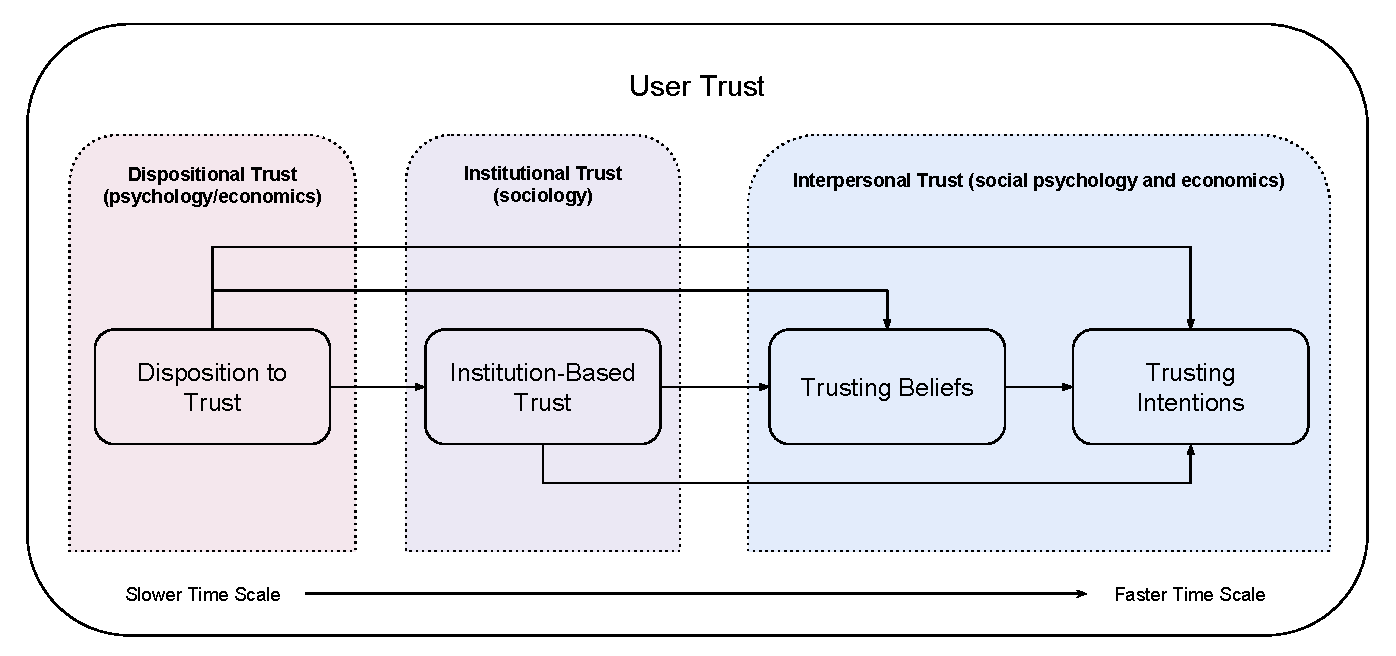
\includegraphics[width=0.75\textwidth]{Figures/UserTrust}
            \caption{Interdisciplinary trust model proposed by \citet{McKnight2001-fa}. The three main categories are delineated, and corresponding disciplines that are interested are listed within parentheses. Connections indicate a causal relationship. The suggestion regarding time scales of the development of trust is the author's addition; trust development is discussed more in \cite{Lewicki2006-gp}, and \cite{Lewicki2006-hj}}
            \label{fig:UserTrust}
        \end{figure}

        In the context of AIAs, the components of the three categories from Figure~\ref{fig:UserTrust} are defined as follows:

        \begin{description}
            \item [Disposition to Trust:] The extent to which one displays a consistent tendency to be willing to depend on AIAs in general across a broad spectrum of situations and persons
            \item [Institution-Based Trust:] One believes that regulations are in place that are conducive to situational success in an endeavor
            \item [Trusting Beliefs:] One believes that the AIA has one or more characteristics beneficial to oneself
            \item [Trusting Intentions:] One is willing to depend on, or intends to depend on, the AIA even though one cannot control its every action
        \end{description}

        Each of these main trust components has sub-components defined in Figure~\ref{fig:Assurance_classes}. These components were defined through the compilation of many research studies across research disciplines, and because of this represent the most accurate notion of the components of trust available. These components comprise the principal drivers of trust-related behaviors (TRBs), and as such are the targets at which assurances must be directed.

        \begin{figure}[htbp]
            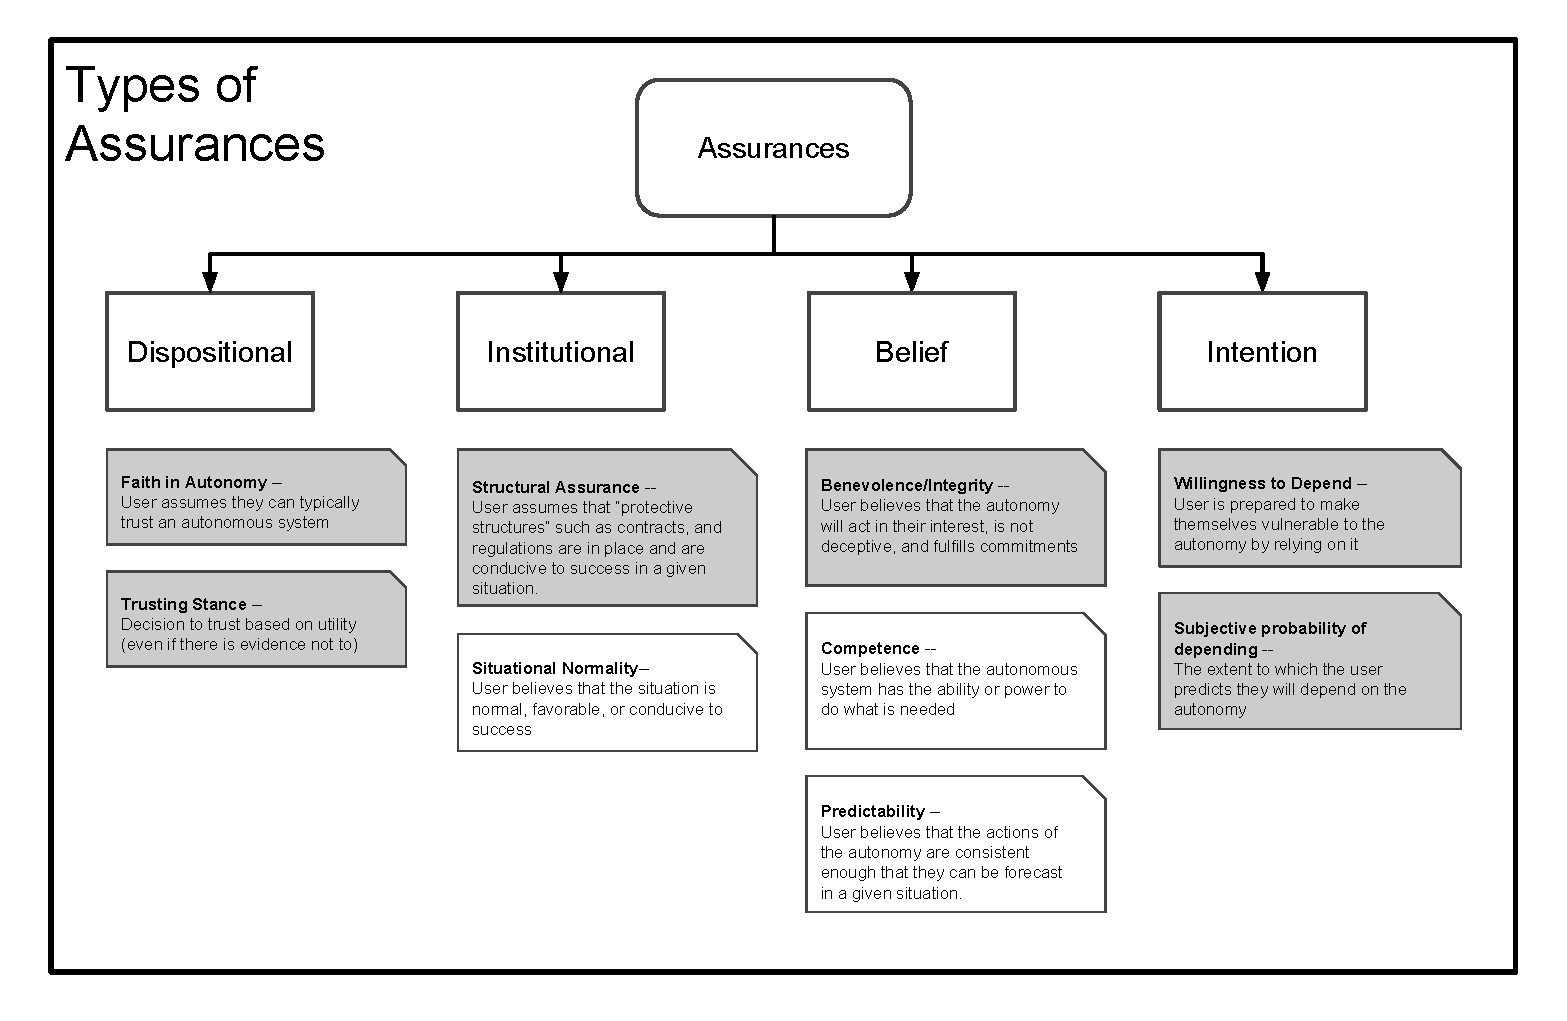
\includegraphics[width=0.8\textwidth]{Figures/Assurances.pdf}%
            \caption{Assurance targets based on the component definitions of the main categories of trust: `Disposition to Trust', `Institution-Based Trust', `Trusting Beliefs', and `Trusting Intentions'}
            \label{fig:Assurance_classes}
        \end{figure}
